\documentclass[12pt,letterpaper]{article}

\author{Jordan Bayles}
\date{}
\title{}
%Usepackage declarations
\usepackage[left=1in,top=1in,right=1in,bottom=1in]{geometry}
\usepackage{fancyhdr}
\usepackage{lastpage}
\usepackage{sectsty}
\usepackage{slashed}
\usepackage{amsmath}
\usepackage{amsfonts}
\usepackage{latexsym}
% Include for use of images
\usepackage{graphicx}
% Include for use of [H] placement specifier
\usepackage{float}
% Include for use of \toprule, \midrule, \bottomrule in tabular env.
\usepackage{booktabs}
% Include for setting spacing between lines
\usepackage{setspace}
%Package usages
\sectionfont{\normalsize}
\subsectionfont{\small}

\setlength{\parindent}{0cm}
%New commands
\newcommand{\comment}[1]{}
\newcommand{\field}[1]{\mathbb{#1}} % requires amsfonts
\newcommand{\pd}[2]{\frac{\partial#1}{\partial#2}}
\newcommand{\cn}[0]{^{\left[\emph{citation needed}\right]}}
\begin{document}

\begin{center}
An analysis of the case where $\theta = 0$
\end{center}
First, we can begin with the derivation of the theta method (TODO: vernacular? 
this wasn't clear online). This begins with the iterative definition of $v$, specifically

\[\frac{v^{n+1} - v^n}{\Delta t} = D v_{zz}^{n+\theta} + \dot{Q}^{n+\theta} \]

Note that if $\theta = 1/2$, this is known as the ``Crank-Nicolson implicit method''
\cite{cj}.

Let $v_{zz}$ (using the partial notation such that $v_{zz} = \pd{^2v}{z^2}$) be defined as

\[ v_{zz}^{n+\theta} := \theta v_{zz}^{n+1} + (1-\theta) v_{zz}^n \]

Then $Q$ can be defined by the relationship

\[ \tau \frac{Q^{n+1} - Q^n}{\Delta t} + Q^n = \epsilon v_{zz}^n \]

And then reformulated for $Q^{n+1}$ as

\[Q^{n+1} = Q^n - \frac{\Delta t}{\tau} Q^n + \frac{\epsilon \Delta t}{\tau} v_{zz}^n \]

Note that this segment of code is where polynomial chaos will shortly be
implemented. Now that the $n+1$th value of $Q$ has been found, a simple finite difference
can be utilized in order to find its time derivative:

\[ \dot{Q}^{n+1/2} = \frac{Q^{n+1} - Q^n}{\Delta t} \]

Finally, this new data can be utilized to solve for the $n+1$th value of $v$, specifically
in the form of

\[v^{n+1} = v^n + \theta D \Delta t A v^{n+1} + (1-\theta) D \Delta t A v^n
  + \Delta t \dot{Q}^{n+1/2} \]

However this is not in its final form, and can be simplified slightly further in order
to reach usability:

\[v^{n+1} = (I-\theta D \Delta t A)^{-1}
\left[v^n + (1-\theta) D \Delta t A v^n + \Delta t \dot{Q}^{n+1/2} \right] \]

We can then analyze the special case where $\theta = 0$. In this instance, $v^{n+1}$
can be written as (using the fact that the identity matrix is its own inverse)
\[v^{n+1} = \left[v^n + D \Delta t A v^n + \Delta t \dot{Q}^{n+1/2} \right] \]

Which is the same as the case in which the theta method is not implemented, with the
definition $D = \kappa H_A G_{\infty}$ (TODO: is this the same?):

\[ v^{n+1} = v^n + \Delta t D v_{zz}^n + \Delta t \kappa H_A \dot{Q}^{n+1/2} \]

\subsection{Advantage of using Crank-Nicolson}
In the case where $\theta = 0$, the Courant-Friedrichs-Lewy condition (CFL condition)
applies as a necessary condition for convergence (due to the fact that we are solving
partial differential equations numerically by finite differences), specifically following
a second order nonlinear finite difference, of the form

\[ \frac{\Delta t}{(\Delta x)^2} < C_u \]

When time steps larger than this calculated value are utilized, the output results
become unstable:
\begin{figure}[H]
	\centering
	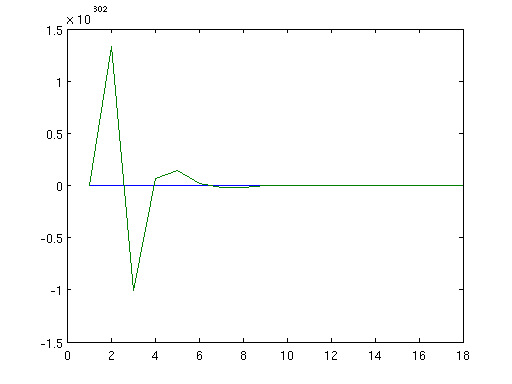
\includegraphics[scale=1]{unstable.png}
	\caption{An example of usage of an overly large time step $\Delta t$}
\end{figure}

Which, in this specific case, $\Delta t$ becomes

\[ \Delta t = \frac{(\Delta z)^2}{ 2 \kappa H_A G_{\infty}} \]

Furthermore, a safety factor$\cn$ is commonly used in order to ensure stability of
the time step. When set to 0.9, this is called the Mingham safety factor$\cn$
\begin{thebibliography}{1}
\bibitem{cj} Crank, J., Nicolson, P.: A practical method for numerical evaluation
of solutions of partial differential equations of the heat conduction type. 
Proceedings of the Cambridge Philosophical Society 43, 50–64 (1947)
\end{thebibliography}
\end{document}
